\documentclass[conference]{IEEEtran}
\IEEEoverridecommandlockouts
% The preceding line is only needed to identify funding in the first footnote. If that is unneeded, please comment it out.
\usepackage{cite}
\usepackage{amsmath,amssymb,amsfonts}
\usepackage{algorithmic}
\usepackage{graphicx}
\usepackage{textcomp}
\usepackage{xcolor}
\usepackage{subcaption}
\def\BibTeX{{\rm B\kern-.05em{\sc i\kern-.025em b}\kern-.08em
    T\kern-.1667em\lower.7ex\hbox{E}\kern-.125emX}}
\begin{document}

\title{Using Generative Adversarial Networks for Textile Design Generation}

    
\author{\IEEEauthorblockN{Shams Arfeen}
\IEEEauthorblockA{
Department of Computer Science \\
Habib Univeristy - Karachi, Pakistan \\
sa05169@st.habib.edu.pk}
\and
\IEEEauthorblockN{Omema Ahmed}
\IEEEauthorblockA{
Department of Computer Science \\
Habib Univeristy - Karachi, Pakistan \\
oa04320@st.habib.edu.pk}
\and
\IEEEauthorblockN{Muhammad Munawwar Anwar}
\IEEEauthorblockA{
Department of Computer Science \\
Habib Univeristy - Karachi, Pakistan \\
ma04289@st.habib.edu.pk}
}


\maketitle

\begin{abstract}
Deep generative models have recently played an important role in the growth of artificial intelligence in a variety of fields that need creativity. Despite its success, the generation of textile patterns is still largely unexplored. One possible explanation is that there is no publicly available data set large enough to train models on. However, research in this area can be useful because fashion designers can take up to several weeks to form a new design as they need inspirations and rely on a human's creativity, but a trained GAN model can generate thousands of designs per day without the need of any human intervention. Furthermore, the use of GANs to generate fabric patterns from traditional Pakistani culture is an untapped field of research. In this research, we will be using DCGANs to generate fabric designs that are representative of Pakistani culture. In addition, we will compare the performance of DCGAN's with StyleGAN and Variational Autoencoders. (VAE)

\end{abstract}

\begin{IEEEkeywords}
Generative Adversarial Network, Textile Patterns, Style Generative Adversarial Network, Pakistani Culture
\end{IEEEkeywords}

\section{INTRODUCTION}

Deep generative models have been crucial in the growth of artificial intelligence in a variety of disciplines that need creativity. One of the most extensively used generative models is generative adversarial networks (GAN) \cite{b5}. Generative adversarial networks are generative models that consists of one or more neural networks. The generator and the discriminator are what make up a of a neural network, where the former generators samples, starting from a random noise and the latter checks and classifies that image as either fake or real. The role of a generator is to minimize the probability of the discriminator to classify an image as fake. At the end of this process, the generator should be capable enough to produce images that are not distinguishable from the original dataset. Many models have been proposed to stabilize the training and improve the image quality. 
\\\\Many disciplines are currently adopting GANs to provide high-quality outcomes for a range of tasks. GANs have also been widely used in computer vision for problems such as image-to-image translation, text-to-image translation, and super-resolution \cite{b6},\cite{b7},\cite{b8},\cite{b9}. GANs have also been utilised for image retrieval, the generation of synthetic data for deep learning tasks, image restoration, and surveillance.

\\\\Fashion is the most recent sector to be transformed by computer vision. The industry is now benefiting from breakthroughs such as neural style transfer \cite{b11}, which utilises CNN to create synthetic customized clothes, and virtual try-on systems, which can generate a realistic image of the person with the desired clothes and posture. In the fashion business, generative models, namely GANs, are widely used. There are other applications such as producing model photos with customized clothing, SwapNet is an algorithm that transfers clothes from one person's image to another irrespective of body location and shape while using GANs \cite{b12}.

Textile industry has been the rampart of Pakistan's economy. It contributes more than 60\% to the total export earnings of the country, accounts for 46\% of the total manufacturing and provides employment to 38\% of the manufacturing labor force and 9\% of GDP \cite{b1}. However, fashion design in Pakistan is more or less an entirely manual process, with little to no automation involved. It requires hours of manual labor to design a prototype pattern, and it goes through multiple iterations and feedback loops to get it finalized. The pattern itself also has to be designed from scratch, and its quality is entirely contingent upon the human designer. 

There are many already designed textile prints freely available on the internet, that have been made by expert professionals. The textile design business can benefit from applying machine learning to learn pattern style and, as a result, develop new patterns. However, recent art generation techniques suffer a number of problems and the research is continuously opening new challenges, for e.g., high resolution, greater fidelity in the generated art, diversity in the output images, control over image features, disentangling the desired features, etc.

This paper aims to address the problem of generating new textile patterns by combining machine intelligence into a creative task of generating aesthetically appealing textile designs for local cultures. Our project's main focus is on locally designed fabric patterns, which will be used to generate new designs following similar style as that of our local prints.

\section{LITERATURE REVIEW}
GANs were initially presented in 2014, and since then, they have been a popular tool for state-of-the-art image synthesis. However, early GAN models suffered from model collapse, training instability, and diminishing gradients. Newer models have been proposed in an attempt to address these concerns. Deep convolution networks were introduced in GANs in 2015, and they have subsequently found widespread use, resulting in sharper pictures \cite{b13}.

\begin{figure}[ht]
\begin{subfigure}{.5\textwidth}
  \centering
  % include first image
  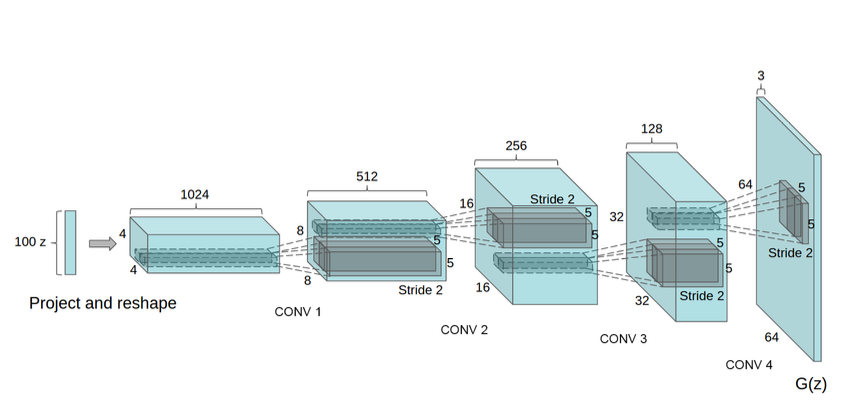
\includegraphics[width=0.8\linewidth]{IEEE/Models/DCAN_generator.png}  
  \caption{DCGAN Generator}
  \label{fig:sub-first}
\end{subfigure}
\begin{subfigure}{.5\textwidth}
  \centering
  % include second image
  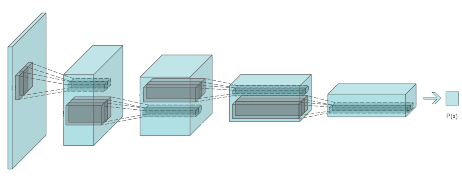
\includegraphics[width=0.8\linewidth]{IEEE/Models/DCAN_discriminator.png}  
  \caption{DCGAN Discriminator}
  \label{fig:sub-second}
\end{subfigure}
\caption{DCGAN Architecture}
\label{fig:fig}
\end{figure}



Wasserstein-GANs (WGANs) were introduced in 2017 and employ the Wasserstein distance as a loss function rather than the standard Jensen-Shannon divergence. WGANs seek to address both model collapse and vanishing gradients \cite{b14}. In 2018, Relativistic GANs were introduced. These were based on the idea that as the discriminator's probability of classifying fake samples as real increases, its probability of classifying real data as real should decrease \cite{b15}. This idea would improve the quality of the generated samples, and would also stabilize training of the model.
As earlier GAN models required hundreds of thousands of images as the training dataset for the model to work, the newer datasets might achieve same or even better results with much fewer data .In 2019, StyleGANs, a style-based architecture that uses an adaptive discriminator augmentation technique to stabilize training while training with restricted data sets, was then developed \cite{b16}.

\begin{figure}[h]
    \centering
    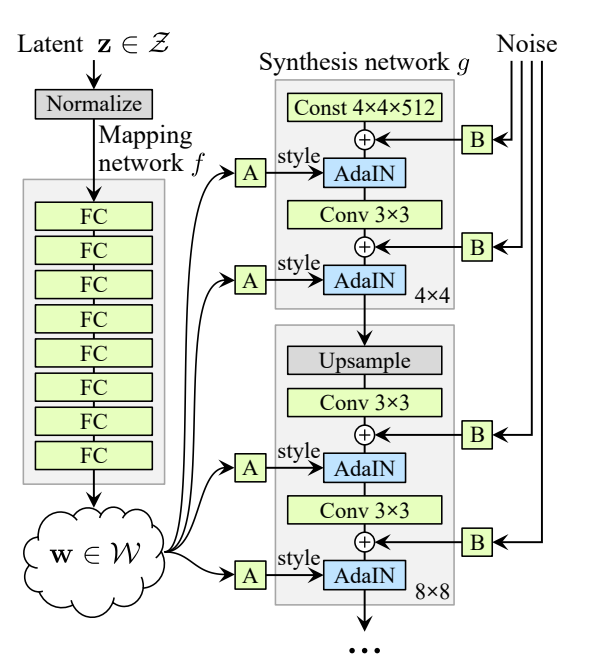
\includegraphics[width=0.5\linewidth]{StyleGAN.PNG}\\
 
    \caption{Style-based Generator Architecture}
    \label{fig:my_label}
\end{figure}

Attempts have previously been made to classify textile design patterns using GANs \cite{b2}, where the performance of image generative models like Wasserstein Generative Adversarial Networks Gradient Penalty (WGANs GP), Deep Convolutional GANs (DCGANs) and Convolutional Variational Autoencoders (CVAEs) for different classes of textile patterns were compared. Moreover, a method of the generation of clothing images for pattern makers using Progressive Growing of GANs (P-GANs) has also been proposed \cite{b4}. Some of these techniques have focused on improving the discriminator network e.g., using multiple discriminators, multi-resolution discrimination, or self-attention. On the generator, the focus was mostly on the shape of the input space or the exact distribution in the input space using clustering, Gaussian mixture models, and encoursing convexity in the models.

In another attempt \cite{b3}, GANs were used for design inspiration. However, these were limited to western-wear and the results generated new t-shirts, jackets and handbags.

Another popular deep learning based generative model that has gained popularity over the year ar Variational Autoenocder (VAEs).  In a VAE, the input data is sampled from a parametrized distribution, and the encoder and decoder are jointly trained so that the output minimises a reconstruction error in the sense of the Kullback-Leibler (KL) divergence between the parametric posterior and the true posterior.

\begin{figure}[h]
    \centering
    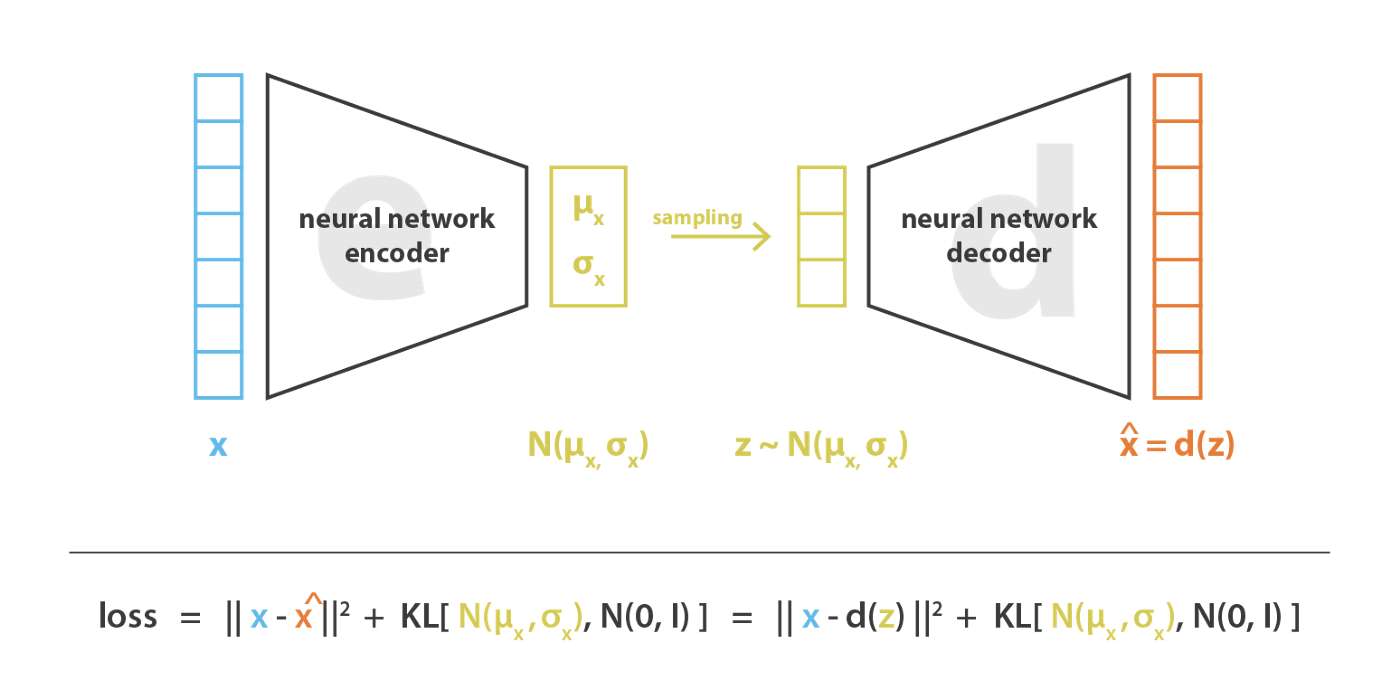
\includegraphics[width=\linewidth]{IEEE/Models/VAE.png}\\
 
    \caption{Variational Autoencoder (VAE)}
    \label{fig:my_label}
\end{figure}

Not much work has been done to construct local Pakistani fabric pattern designs using GANs, which is what our paper aims to focus on. 

\section{DATASET}
\subsection{Data Collection}
We will be using the open source dataset of textile prints \cite{b10}. This data set contains about 15K images. Each image is of the size 256 by 256 and belongs to one  of  six different categories; checkered, dotted, floral, solid, striped, zig zag. These images are takes from actual fabrics, and some of them are of low-fidelity. Therefore, we would need to augment our dataset in order to reach the desired number of prints required, and get the expected output from GANs.
\subsection{Data augmentation}
To incorporate our locally designed fabric prints and increase the size of our dataset for training, we will collect data through web-scrapping from online resources of freely available Pakistani fabric prints. Some samples from our dataset are shown below.
    \begin{figure}[h]
          \centering
          {%
            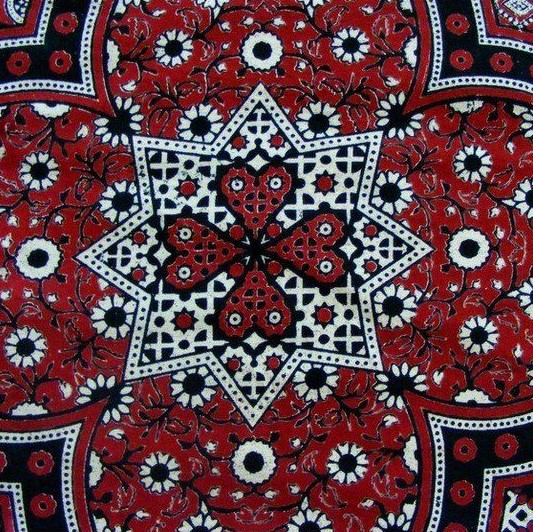
\includegraphics[width=.2\linewidth]{1.jpg}}\quad
          {%
            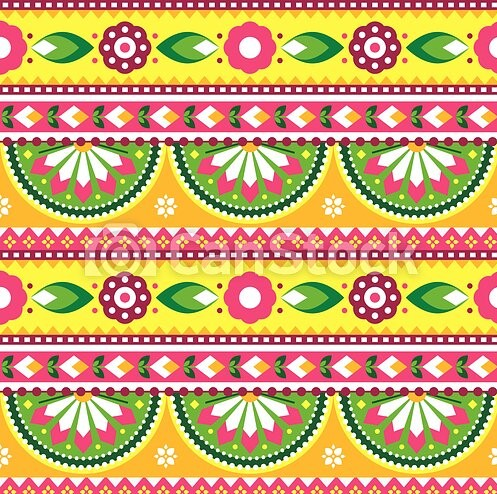
\includegraphics[width=.2\linewidth]{2.jpg}}\quad
          {%
            
\includegraphics[width=.2\linewidth]{3.jpg}}
              \caption{Fabric prints dataset}
        \label{fig:initialchromsome}
    \end{figure}

\section{NOVELTY}
Computational creativity has attracted a lot of attention in the research community. The generation of new creative designs is an arduous task which requires a lot of brain work. One of the most important phases in product manufacturing is design generation. However, not much focus has been put on automating the design generation aspect of the textile industry in Pakistan. \\
All related previous work done in this domain either focused on general fabric patterns or western wear, with no particular focus on our local Pakistani textile industry and its prints. Therefore, to address local fashion industries residing in Pakistan, the aesthetics of our generated patterns will primarily be based on sub continental heritage and designs. In our project, we have mainly focused on Pakistani fabric prints available on the internet by web-scrapping websites that are Indian/Pakistani based. \\
Moreover, for our project we have implemented three different models to check which architecture would give us the most appealing results. 


\section{MODEL \& EXPERIMENTS}

\subsection{Experimental Setup}
We compared the performance of DCGAN, StyleGAN and VAEs by using images of size of 64 by 64 and a dataset containing 2K images. Since DCGAN outperformed the two other models, we trained the further trained the DCGAN on a dataset containing 15K images of size 256 by 256.
\begin{table}[htbp]
\begin{center}
\caption{The parameters used to compare the performance of DCGAN, StyleGAN and VAE.}
\begin{tabular}{|l|l|}
\hline
Parameter                  & Values \\ \hline
Epochs                     & 1000   \\ \hline
Batch Size                 & 24     \\ \hline
Number of   Image Channels & 3      \\ \hline
Learning Rate              & 0.0002 \\ \hline
Latent   Dimension         & 512    \\ \hline
Number of   Images         & 2K     \\ \hline
\end{tabular}%
\end{center}
\label{tab:my-table}
\end{table}
\vfill\null
\begin{table}[htbp]
\begin{center}
\caption{The value of the hyper parameters used to train the final DCGAN model}
\begin{tabular}{|l|l|}
\hline
Parameter                  & Values \\ \hline
Epochs                     & 12,000   \\ \hline
Batch Size                 & 24     \\ \hline
Number of   Image Channels & 3      \\ \hline
Learning Rate              & 0.00002 \\ \hline
Latent   Dimension         & 100    \\ \hline
Number of   Images         & 15K     \\ \hline
\end{tabular}%
\end{center}
\label{tab:my-table1}
\end{table}

\subsection{VAE}
We implemented our VAE model consisting of two neural net models; encoder and the decoder. Our encoder consists of five Convolutional layers followed three dense layers. Each Convolutional layer is followed by batch normalisation. The activation function function used between each Convolutional layer is ReLU. Our decoder consists of one dense layer followed by Upsample layers. Each Upsample layer is followed by Conv2D and Batch Normalization. The activation between each upsampling layer is ReLU.


\begin{figure}[htbp]
\centerline{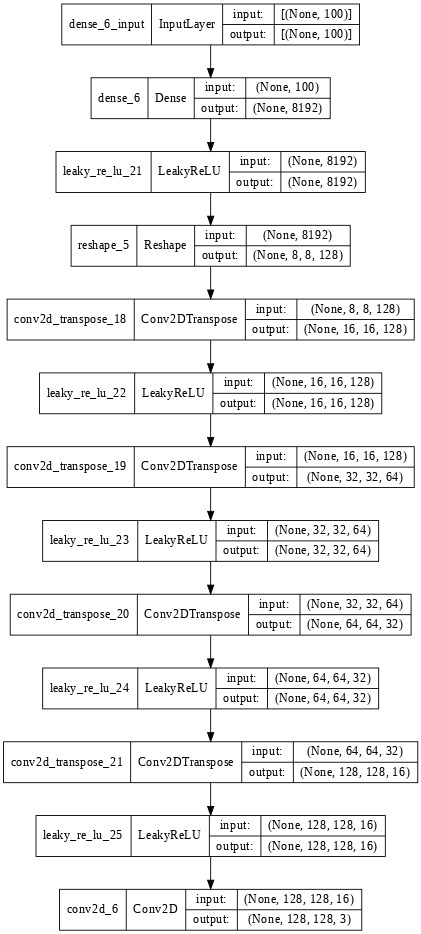
\includegraphics[width=0.2\textwidth]{IEEE/Models/VAE_D_64.jpeg}}
\caption{Architecture of VAE - Decoder}
\label{fig}
\end{figure}
\break
\begin{figure}[htbp]
\centerline{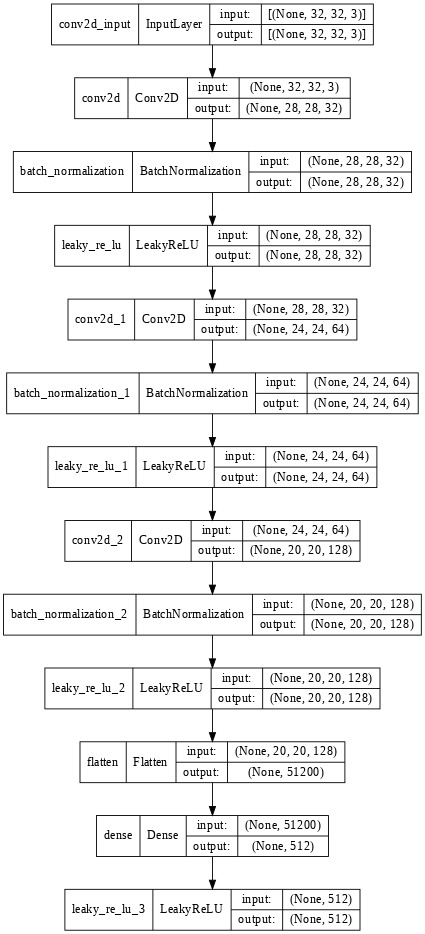
\includegraphics[width=0.2\textwidth]{IEEE/Models/VAE_E_64.jpeg}}
\caption{Architecture of VAE - Encoder}
\label{fig}
\end{figure}
\subsection{StyleGAN}
We have implemented our StyleGAN model the same as the original model that was presented so no custom diagrams have been included.
\subsection{DCGAN}.

Each of our DCGAN model consisting of two neural net models; generator and  discriminator. Our generator model consists of five Conv2DTranspose layers with one Dense Layer with LeakyRelu activation function between these layers, and tanh function as the activation function for the last layer. Our discriminator consists of six Conv2DTranspose Layer, one Dense Layer with LeakyRelu activation function between these layers, and sigmoid function as the activation function for the last layer. \\ The structure of the DCGAN which works on 64 by 64 images is similar to the DCGAN which works on 256 by 256 images. The generator now conists of thee Conv2DTranspose layers instead of five and the discriminator consists of four instead of six layers.

\begin{figure}[h!]
\centerline{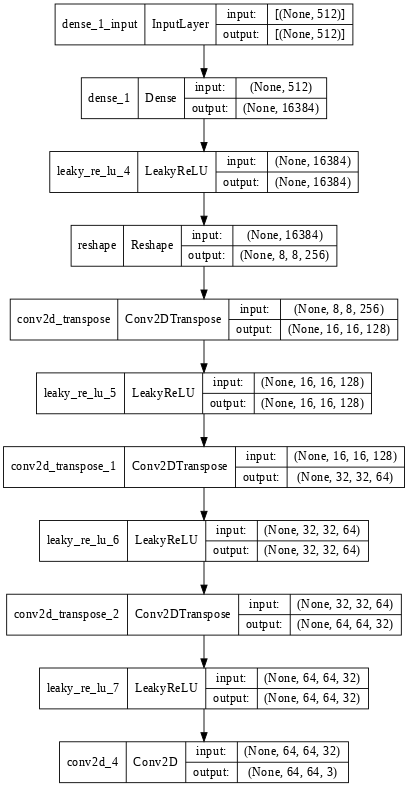
\includegraphics[width=0.1\textwidth]{IEEE/Models/DCGAN_G_64.png}}
\caption{Architecture of DCGAN model(64 by 64) - Generator}
\label{fig}
\end{figure}

\begin{figure}[h!]
\centerline{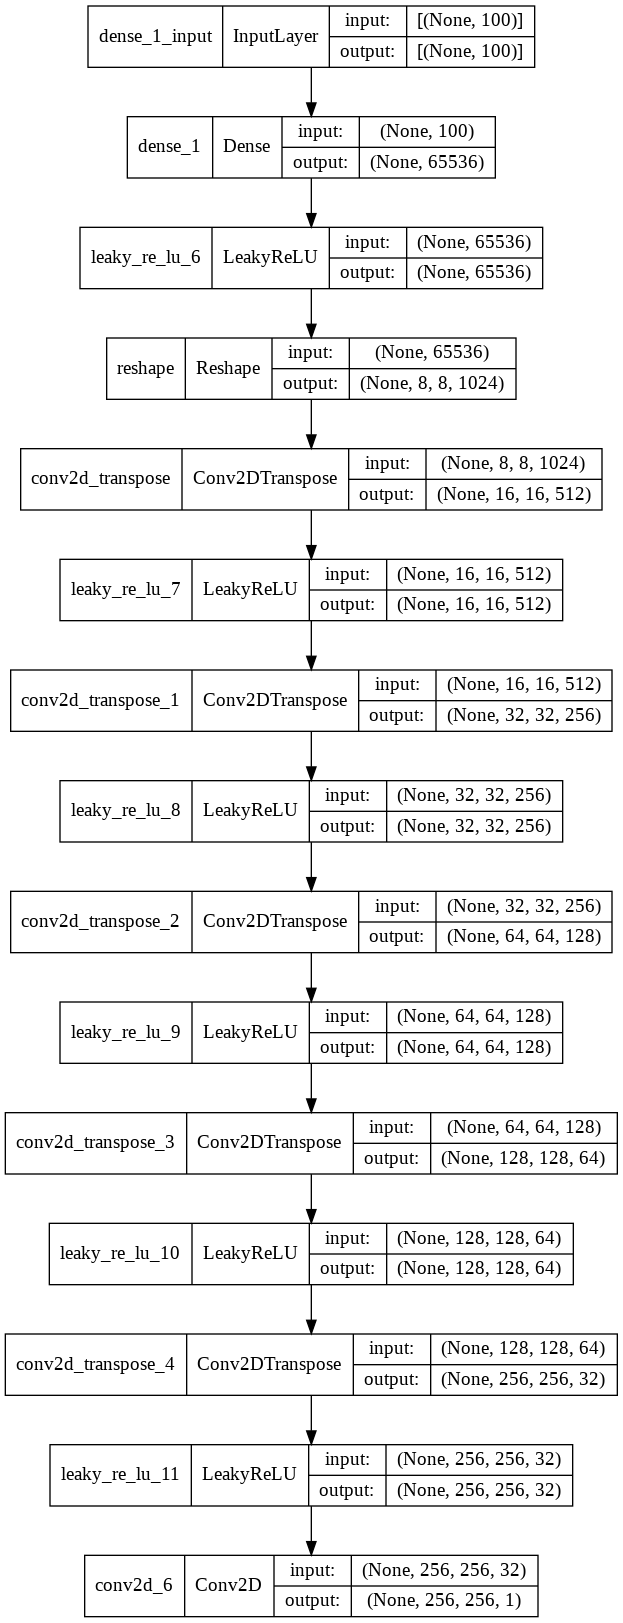
\includegraphics[width=0.1\textwidth]{IEEE/Generator_model.png}}
\caption{Architecture of DCGAN model(256 by 256) - Generator}
\label{fig}
\end{figure}
\newpage

\begin{figure}[h!]
\centerline{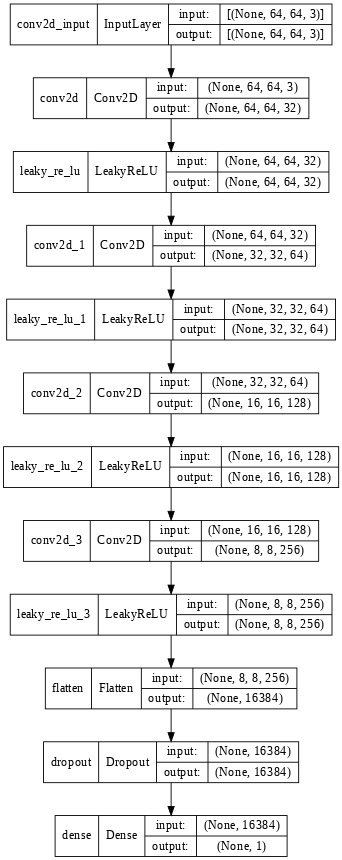
\includegraphics[width=0.1\textwidth]{IEEE/Models/DCGAN_D_64.png}}
\caption{Architecture of DCGAN model(64 by 64) - Discriminator}
\label{fig}
\end{figure}


\begin{figure}[h!]
\centerline{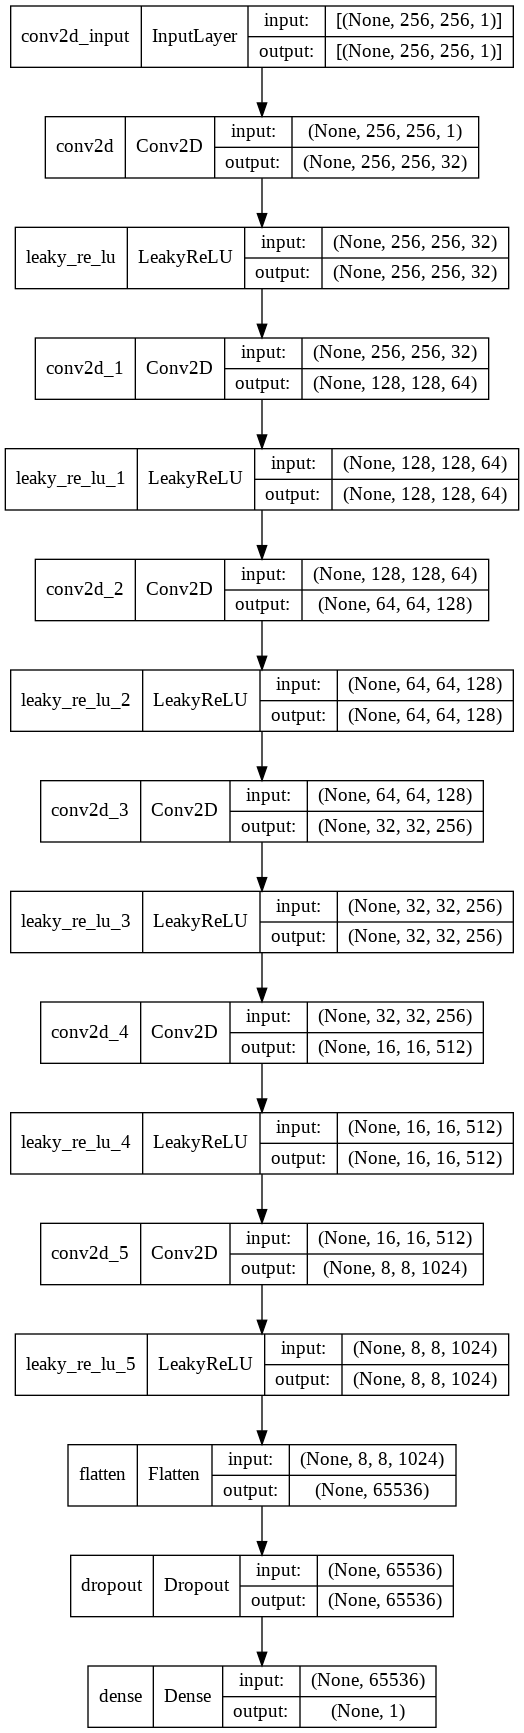
\includegraphics[width=0.1\textwidth]{IEEE/Discriminator_model.png}}
\caption{Architecture of DCGAN model(256 by 256) - Discriminator}
\label{fig}
\end{figure}

\section{Results \& Discussion}
\subsection{VAE}
The results that were generated by the VAE were blurry and lacked any distinct shape. However, they contained some form of resemblance to the fabric patterns that were presented in the dataset.
\begin{figure}[h!]
\centerline{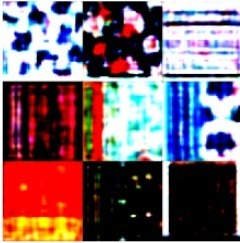
\includegraphics[width=0.2\textwidth]{IEEE/Models/VAE_Results.jpeg}}
\caption{Results generated by the VAE - 64 by 64 Image}
\label{fig}
\end{figure}

\subsection{StyleGAN}
The results that were generated by the StyleGAN were quite blur and lacked any distinct pattern or shape.
\begin{figure}[h!]
\centerline{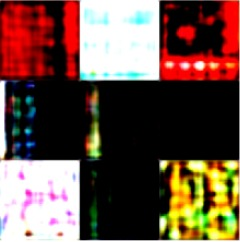
\includegraphics[width=0.2\textwidth]{IEEE/Models/StyleGAN_64_results.jpeg}}
\caption{Results generated by the StyleGAN - 64 by 64 Image}
\label{fig}
\end{figure}

\subsection{DCGAN}
The results that were generated by the DCGAN were also blur but contained less variance and noise as compared to the outputs generated by the VAE and StyleGAN model.
\begin{figure}[h!]
\centerline{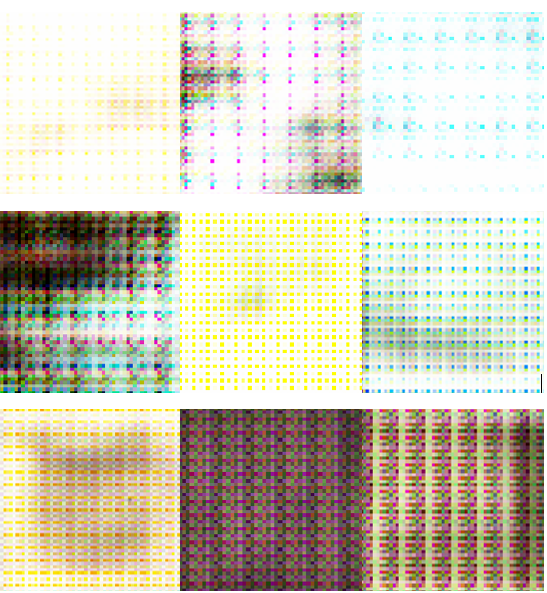
\includegraphics[width=0.2\textwidth]{IEEE/Models/DCGAN_Results_64.png}}
\caption{Results generated by the DCGAN - 64 by 64 Image}
\label{fig}
\end{figure}

\subsection{Discussion}
Our DCGAN model outperformed the StyleGAN and VAE model. Consequently, we trained the DCGAN on a dataset with 15K images of size 256 by 256.  The results can be seen in Figure \ref{fig:initialchromsome}. 

\begin{figure}[h]
          \centering
          {%
            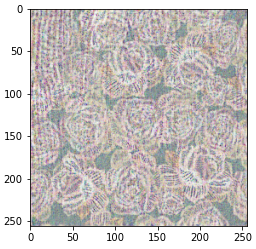
\includegraphics[width=.2\linewidth]{IEEE/output 19.png}}\quad
          {%
            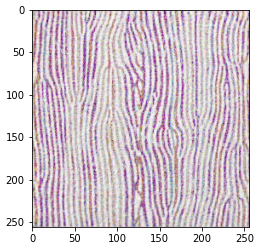
\includegraphics[width=.2\linewidth]{IEEE/output 4500.png}}\quad
          {%
            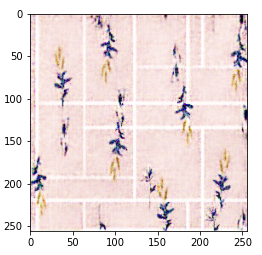
\includegraphics[width=.2\linewidth]{IEEE/output 5500.png}}
        \label{fig:initialchromsome}
\end{figure}
\begin{figure}[h]
          \centering
          {%
            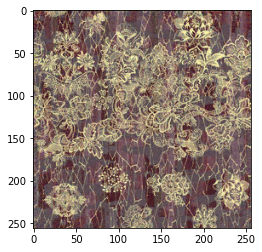
\includegraphics[width=.2\linewidth]{IEEE/output1.png}}\quad
          {%
            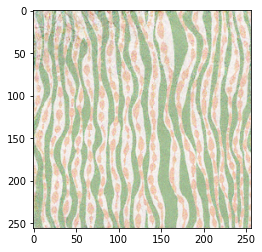
\includegraphics[width=.2\linewidth]{IEEE/output15.png}}\quad
          {%
            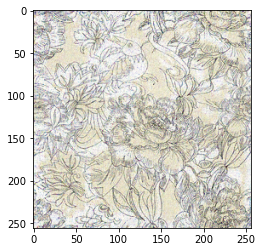
\includegraphics[width=.2\linewidth]{IEEE/output2.png}}
              \caption{Results generated by the DCGAN - 256 by 256 Image.}
        \label{fig:initialchromsome}
\end{figure}

\begin{figure}[h!]
    \centering
    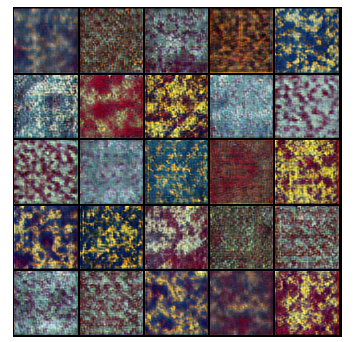
\includegraphics[width=0.5\linewidth]{IEEE/Models/DCAN_Previous.png}
    \caption{Previous Results \cite{inproceedings}. DCGAN generating image of size 64 by 64 with noise.}
    \label{fig:my_label}
\end{figure}
Our results are an improvement because the previous models generated low-resolution images of size 64 by 64 but our model produces high resolution images of size 256 by 256. Increasing the size of images has also reduced the noise that was found in the previous results. In addition, the results produced by our VAE model were similar to the results produced by the previous VAE models. \\
One explanation for these results is that the DCGAN suffers from over fitting. Consequently, the patterns that are generated are sharp but have a low variance. On the other hand, VAE and StyleGAN models try to learn all the different patterns in the dataset and then combine these patterns to generate a new pattern. However, since the training dataset has a high variance when these different patterns are mixed the resulting image has noise.

\section{Future Work}
In our project, we focused on an architecture centric approach; we implemented the model that we want to use first and then collected data for it. To get better results, a data centric approach should be taken to solve this problem of automating the process of textile designs, as we need to implement such a model that works best on the type of data available to us. \\
Moreover, our scrapped dataset has a lot of variance in it. All our selected patterns used to train our model on are each very different from one another. There is little to no similarity between these designs, due to which its harder for our model to learn features. To overcome this problem and get better results, a dataset with fewer variance needs to be collected for such a problem. For example, focusing only on Ajrak prints or Geometric prints would be ideal. \\

Furthermore, there is no way to measure the aesthetic value of design using mathematical formulas. The evaluation of a good design is what appeals to the eye, and its not possible that all the designs that our model generates would be aesthetically pleasing. Therefore, working on calculating the aesthetic value for each design, or incorporating human input to select and reject the generated designs could be something to work on in future.
\\
Due to our limitations in this project, we could not train our model for longer periods of time. Training these models for larger periods of time increases the model's ability to learn new features. To make this possible, use of a GPU to train the model would help for future work in this domain.  \\



\bibliography{references}
\bibliographystyle{plain}

\end{document}


%%%%%%%%%%%%%%%% Things to be done
% Update Abstract (Done)
% Add VAE in Literature Review (Done)
% Data size need (Done)
% Experimental Results
% Add Model Diagrams for each case.
% Parameters + Explanation of the results
% StyleGAN
% DCGAN
% VAE
% Conclusion
% - DCGAN performed than other GANs
% However it was overfitting on the a particular patterns
% VAE and StyleGAN were tryig to mix multiple patterns so image contained noise
% Selecting a dataset which has a fewer variance and take a data centric appproach rather than a model centric approach.

% Two things 
% 1. Write Novelty (Done)
% 2. Give me four images 64 - VAE, StyleGAN, DCGAN at 1000 epochs
% 